\section{Original Sequential Baseline}
\label{sec:original-baseline}

\subsection{Measurement Procedure}
The implementation was developed and small tests were measured on \texttt{louie}, a KVM virtual
machine exposing four logical CPUs with an Intel Core i3-12100F
with 16GiB of RAM.
Compilation used GNU g++ 14.2.0, CMake 3.31.6, and Release flags
\texttt{-O3 -DNDEBUG -std=gnu++20}.

The tested square matrix dimensions were $N=64$, $128$, and $256$.
For each dimension, the executable was configured and built once before
three separate measured executions. Each execution used seed 123456 and
the field of order $11^3=1331$, with defining polynomial $x^3+x+4$.
The build command and the first measurement command used for $N=256$
are recorded below as an example, other dimensions just substitute 
the size in the \texttt{-DALGEBRA\_ASSIGNMENT\_SIZE} option and the log file name.

\begingroup
\scriptsize
\begin{verbatim}
cmake -S . -B build \
  -DCMAKE_BUILD_TYPE=Release \
  -DALGEBRA_ASSIGNMENT_SIZE=256 \
  && cmake --build build --parallel

/usr/bin/time -v \
  ./build/src/algebra_determinants \
  2>&1 | tee original-256-run1.log
\end{verbatim}
\endgroup

Only the executable was timed, not the build. The combined output retained
the field metadata, determinant coefficients, correctness check, application
phase timings, and GNU Time resource measurements. All nine runs returned
exit status zero and verified $\det(AB)=\det(A)\det(B)$. For each dimension,
the determinant coefficients agreed across all three repetitions.

\subsection{Runtime and Peak Memory}
Table~\ref{tab:original-baseline} reports the median GNU Time elapsed wall
time, the median application-reported total, and the largest peak resident
set size among the three repetitions. 
The application total uses its own steady-clock interval.

\begin{table}[tb]
\centering
\caption{Original sequential baseline over three runs per dimension}
\label{tab:original-baseline}
\begin{tabular}{rrrr}
\hline
$N$ & Wall (s) & App total (s) & Peak RSS (MiB) \\
\hline
64 & 0.15 & 0.151263 & 4.684 \\
128 & 1.10 & 1.102611 & 7.121 \\
256 & 8.73 & 8.728325 & 17.637 \\
\hline
\end{tabular}
\end{table}

Application total times ranged from 0.147525 to 0.151736~s at $N=64$,
1.098483 to 1.110965~s at $N=128$, and 8.640466 to 8.730073~s at $N=256$.
Doubling the dimension from 128 to 256 increased the median application
total by approximately 7.92 times, consistent with the cubic arithmetic
work of matrix multiplication and elimination.

Table~\ref{tab:original-phases} separates multiplication from the three
determinant computations. Each timing column is summarized independently.
For $N=256$, the median combined time for calculating all three 
determinants was 4.273438 seconds, while matrix multiplication took 4.418723 seconds. 
This indicates that multiplication took slightly longer than the three determinant calculations combined.

\begin{table}[tb]
\centering
\caption{Median original phase times in seconds}
\label{tab:original-phases}
\begin{tabular}{rrrrr}
\hline
$N$ & Product & $\det(A)$ & $\det(B)$ & $\det(C)$ \\
\hline
64 & 0.0797 & 0.0227 & 0.0230 & 0.0228 \\
128 & 0.5468 & 0.1794 & 0.1805 & 0.1801 \\
256 & 4.4187 & 1.4143 & 1.4193 & 1.4212 \\
\hline
\end{tabular}
\end{table}

These results establish the original runtime and memory baseline on the
local host. Per-run measurements, summary statistics, and environment metadata
are retained in the repository alongside the raw logs.

\subsection{Function-Level Profile}
\label{sec:original-profile}
A separate run at $N=256$ used GNU gprof 2.44, adding \texttt{-pg -g} during
compilation and \texttt{-pg} during linking. The program retained Release
optimization, the same seed, and the original arithmetic. It verified the same
determinants and multiplicative identity. Its profiling data and text report
were generated with the following commands:

\begingroup
\scriptsize
\begin{verbatim}
./build/src/algebra_determinants \
  > original-256-profile-run.log
gprof -b ./build/src/algebra_determinants \
  gmon.out > original-256-profile.txt
\end{verbatim}
\endgroup

Fig.~\ref{fig:original-profile} shows the flat profile's sampled self-time
shares. Self time excludes separately reported callees~\cite{gprof-flat}.
Matrix multiplication accounted for 49.71\%, the determinant function for
35.19\%, and polynomial division/remainder for 12.13\%. The profiler recorded
50,233,382 calls to the polynomial \texttt{divmod} routine. The small remaining
shares were attributed to the \texttt{\_init} symbol and random-generator state
refresh.

\begin{figure}[tb]
\centering
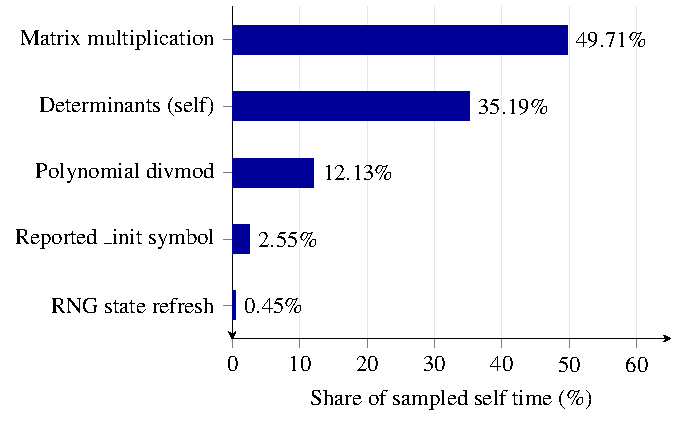
\includegraphics[width=\columnwidth]{figures/original-profile.pdf}
\caption{Reported sampled self-time shares for the optimized, instrumented
$256\times256$ original run. Values describe profiler samples, not wall-time
fractions; inlined arithmetic is attributed to its enclosing function.}
\label{fig:original-profile}
\end{figure}
